\subsection{Single course, single start date, single weekly pattern}

This case can be solved in polynomial time. Indeed, it is a simple case of a maximum-cost maximum-flow problem. Specifically, if we let \begin{itemize}
\item $p$ be the number of professors,
\item $d$ be the number of days,
\item $m$ be the number of roles, and
\item $n'_{i, k}$ be the number of professors of role $k$ that are needed on whichever class falls on the $i$th day
\end{itemize}

we can create the following flow network, where capacities are in blue, and costs are in red:

\vspace{10pt}

\begin{center}
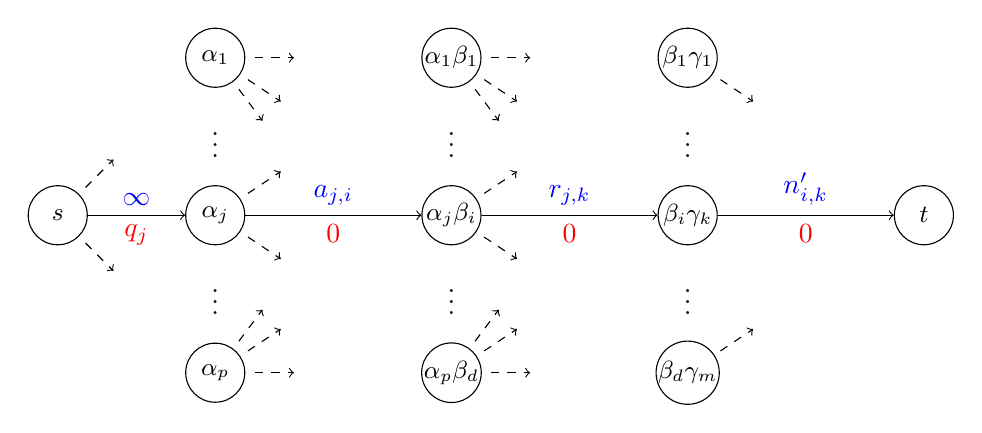
\begin{tikzpicture}
\usetikzlibrary{calc}

\tikzstyle{v}=[draw, circle, inner sep=0pt, font=\small, align=center, minimum size=0.75cm];
\tikzstyle{e}=[->, dashed];
\node[v] (s) at (1, 1) {$s$};
\node[v] (p_j) at (3, 1) {$\alpha_j$};
\node (d1) at (3, 2) {$\vdots$};
\node (d2) at (3, 0) {$\vdots$};
\node[v] (d3) at (3, 3) {$\alpha_1$};
\node[v] (d4) at (3, -1) {$\alpha_p$};

\node[v] (p_jd_i) at (6, 1) {$\alpha_j \beta_i$};
\node (d5) at (6, 0) {$\vdots$};
\node (d6) at (6, 2) {$\vdots$};
\node[v] (d7) at (6, 3) {$\alpha_1 \beta_1$};
\node[v] (d8) at (6, -1) {$\alpha_p \beta_d$};

\node[v] (d_ir_k) at (9, 1) {$\beta_i \gamma_k$};
\node (d9) at (9, 0) {$\vdots$};
\node (d10) at (9, 2) {$\vdots$};
\node[v] (d11) at (9, 3) {$\beta_1 \gamma_1$};
\node[v] (d12) at (9, -1) {$\beta_d \gamma_m$};

\node[v] (t) at (12, 1) {$t$};

\draw[->] (s) to node[above,blue] {$\infty$} node[below,red] {$q_j$} (p_j);
\draw[e] ($(s)!0.5cm!(d3)$) -> ($(s)!1cm!(d3)$);
\draw[e] ($(s)!0.5cm!(d4)$) -> ($(s)!1cm!(d4)$);
\draw[->] (p_j) to node[above,blue] {$a_{j, i}$} node[below,red] {$0$} (p_jd_i);

\draw[e] ($(d3)!0.5cm!(d7)$) -> ($(d3)!1cm!(d7)$);
\draw[e] ($(d3)!0.5cm!(p_jd_i)$) -> ($(d3)!1cm!(p_jd_i)$);
\draw[e] ($(d3)!0.5cm!(d8)$) -> ($(d3)!1cm!(d8)$);

\draw[e] ($(d4)!0.5cm!(d7)$) -> ($(d4)!1cm!(d7)$);
\draw[e] ($(d4)!0.5cm!(p_jd_i)$) -> ($(d4)!1cm!(p_jd_i)$);
\draw[e] ($(d4)!0.5cm!(d8)$) -> ($(d4)!1cm!(d8)$);

\draw[e] ($(p_j)!0.5cm!(d7)$) -> ($(p_j)!1cm!(d7)$);
\draw[e] ($(p_j)!0.5cm!(d8)$) -> ($(p_j)!1cm!(d8)$);

\draw[->] (p_jd_i) to node[above,blue] {$r_{j, k}$} node[below,red] {$0$} (d_ir_k);

\draw[e] ($(d7)!0.5cm!(d11)$) -> ($(d7)!1cm!(d11)$);
\draw[e] ($(d7)!0.5cm!(d_ir_k)$) -> ($(d7)!1cm!(d_ir_k)$);
\draw[e] ($(d7)!0.5cm!(d12)$) -> ($(d7)!1cm!(d12)$);
\draw[e] ($(d8)!0.5cm!(d11)$) -> ($(d8)!1cm!(d11)$);
\draw[e] ($(d8)!0.5cm!(d_ir_k)$) -> ($(d8)!1cm!(d_ir_k)$);
\draw[e] ($(d8)!0.5cm!(d12)$) -> ($(d8)!1cm!(d12)$);
\draw[e] ($(p_jd_i)!0.5cm!(d11)$) -> ($(p_jd_i)!1cm!(d11)$);
\draw[e] ($(p_jd_i)!0.5cm!(d12)$) -> ($(p_jd_i)!1cm!(d12)$);

\draw[->] (d_ir_k) to node[above,blue] {$n'_{i, k}$} node[below,red] {$0$} (t);
\draw[e] ($(d11)!0.5cm!(t)$) -> ($(d11)!1cm!(t)$);
\draw[e] ($(d12)!0.5cm!(t)$) -> ($(d12)!1cm!(t)$);
\end{tikzpicture}
\end{center}

Formally, the network is $G = (V, E)$, with

\begin{align*}
V = &\{s\} \cup \{t\}\\
&\cup \{\alpha_j \mid 1 \le j \le p\}\\
&\cup \{\alpha_j \beta_i \mid 1 \le j \le p, 1 \le i \le d\}\\
&\cup \{\beta_i \gamma_k \mid 1 \le i \le d, 1 \le j \le m\}\\
E = &\{(s, \alpha_j)\ \forall\ j\}\\
    &\cup \{(\alpha_j, \alpha_j \beta_i)\ \forall\ i, j \}\\
    &\cup \{(\alpha_j \beta_i, \beta_i \gamma_k)\ \forall\ j, i, k\}\\
    &\cup \{(\beta_i \gamma_k, t)\ \forall\ i, k \}
\end{align*}

capacity function $c:E \to \mathbb{R} \cup \{\infty\}$, such that
\begin{align*}
c(s, \alpha_j) &= \infty\ \forall\ j\\
c(\alpha_j, \alpha_j \beta_i) &= a_{j, i}\ \forall\ i, j\\
c(\alpha_j \beta_i, \beta_i \gamma_k) &= r_{j, k}\ \forall\ i, j, k\\
c(\beta_i \gamma_k, t) &= n'_{i, k}\ \forall\ i, k
\end{align*}

and cost function $w:E \to \mathbb{R}$, such that

$$
w(e) =
\begin{cases}
q_j &\text{ if } e = (s, a_j) \text{ for some }j\\
0 & \text{otherwise}
\end{cases}
$$

We can think of the flow in this network as ``time'' dedicated by a professor at a given day, on a given role. A unit of flow goes from a professor to a given day (only if that professor is available that day), and to a given role (only if the professor could fit that role), and into fulfilling that day's quota for that role.

A professor cannot teach on an unavailable day, since flow can only go from the $j$th professor to the $i$th day if $a_{i, j} = 1$, and only one unit may go through in that case. This last fact ensures a professor cannot work twice in a single day, even under different roles.

He also cannot work in a role that is unavailable to him, since in order for flow to go from $\alpha_j \beta_i$ to $\beta_i \gamma_k$, meaning ``the $j$th professor teaches on the $i$th day'' to ``the $i$th day has one $k$th role position covered'', unless $r_{j, k} = 1$, so one cannot consider an instance of that role covered for that day unless the professor from which that unit of flow came indeed can work in that role.

Lastly, the number of instances of the $k$th role that a given $\beta_i \gamma_k$ needs for the $i$th day can not be greater than $n'_{i, k}$.

A flow $f$ in $G$ will be a valid assignment of professors exactly when $f(s, t) \ge \sum_{i, k} n'_{i, k}$. The constraints going into $t$ guarantee this implies $f(\beta_i \gamma_k, t) = r_{i, k}\ \forall i, k$, which means each day's requirements of each role are met.

In such a solution, if a unit of flow goes from $s$, to $\alpha_j$, through $\alpha_j \beta_i$, then through $\beta_i \gamma_k$, and finally to $t$, we consider that the $j$th professor teaches on the $i$th day with the $k$th role. The quality of this assignment is thus $q_j$.

Furthermore, to obtain an optimal solution, that is, a maximum sum of the qualities of the assignments, we need to maximize the cost of this flow, because this will mean the maximum value of the units going into (hence out of) the $\alpha_j$, which is the quality of the assignments we are making.

Since maximum-cost maximum-flow on $G$ is in $O(poly(|V|, |E|))$, and we can see our $|V|$ and $|E|$ are polynomials in $p, d, m$, we coclude this reduction can be solved in time $O(poly(p, d, m))$, and thus is in \textsc{P}.
